
\documentclass{ppgeesa}

%%%%%%%%%%%%%%%%%%%%%%%%%%%%%%%%%%%%%%%%%%%%%%%%%%%%%%%%%%%%%%%%%%%%%%%%%%%%%%%%%%%%%%%%%%%%%%%%%%%%%%%%%%%%%%%%%

\usepackage[latin1]{inputenc}
\usepackage{graphicx}
\usepackage{hyperref}
\usepackage{tikz}
\usepackage{amsmath}
\usepackage{listings}
\lstset{language=Python}

\lstset{stepnumber=2, frame=single,tabsize=2, breaklines=true, basicstyle=\footnotesize}

\hypersetup{
	colorlinks,
	debug=true,
	linkcolor=black,  %%% cor do tableofcontents, \ref, \footnote, etc
	citecolor=red,  %%% cor do \cite
	urlcolor=blue,   %%% cor do \url e \href
	bookmarksopen=true,
	pdftitle={Modelagem e identifica��o de sistemas},
	pdfauthor={Tassiano Neuhaus},
	pdfsubject={M�todos n�o param�tricos de identifica��o},
	pdfkeywords={Identifica��o de sistemas}
	%pdfpagemode=FullScreen
}

%%%%%%%%%%%%%%%%%%%%%%%%%%%%%%%%%%%%%%%%%%%%%%%%%%%%%%%%%%%%%%%%%%%%%%%%%%%%%%%%%%%%%%%%%%%%%%%%%%%%%%%%%%%%%%%%%


\begin{document}

\title{M�todos n�o param�tricos de identifica��o de sistemas}

\author{Tassiano Neuhaus\\
{\small Universidade Federal do Rio Grande do Sul - Departamento de Engenharia El�trica\\Av. Osvaldo Aranha, 103 - Bairro Bom Fim CEP: 90035-190 - Porto Alegre - RS - Brasil}\\
}%\thanks{Tassiano Neuhaus, tassianors@gmail.com, tel +55-51-91760154}}

\maketitle
\thispagestyle{empty}\pagestyle{empty}

\begin{abstract}
Este trabalho tem por objetivo demonstrar de forma simplificada um caso de uso de modelagem
de sistema por m�todos n�o param�tricos. Ser� apresentado desde a abordagem mais simples, onde
aplica-se simplesmente uma onda senoidal e observa-se a amplitude e a fase da onda produzida na 
sa�da do processo, at� m�todos um pouco mais rebuscado, que buscam minimizar a influ�ncia
do ruido sobre o sistema.

Para isso ser� utilizado um sistema com fun��o de transfer�ncia conhecida, onde ser� aplicado 
um ruido branco de m�dia zero, e ser�o utilizados os m�todos comentados anteriormente para
levantar a fun��o de transfer�ncia do processo sujeito ao ruido.

Ao fim ser� apresentado um comparativo dos resultados obtidos em cada m�todo.
\end{abstract}

\begin{IEEEkeywords}
Identifica��o de sistemas lineares, m�todos n�o param�tricos.
\end{IEEEkeywords}

%===============================================================================
\section{Introdu��o}

Neste trabalho ser� apresentado um sistema de para controle de posi��o angular,
manipulado por um motor de corrente continua (DC). O objetivo principal, � estimar
os valores das vari�veis existentes no modelo escolhido para representar este sistema.

Inicialmente ser� explicado o processo de escolha do modelo que representa a din�mica
deste sistema (Se��o (\ref{sec:modelling})). Ser� explicitado quais considera��es sobre
o sistema foram feitas para se obter o modelo que ser� utilizado nas se��es seguintes, 
para determinar os par�metros.

Em seguida, ser� utilizado o m�todo dos M�nimos quadrados (MQ), para estimar o sistema, 
considerando-se para isso que o ruido sobre o sistema sofre influ�ncia dos mesmos polos
que est�o na planta, ou seja, que o modelo para o sistema se comporta como um modelo ARX.
Nesta mesma se��o (\ref{sec:mmq}) ser� apresentado os resultados para o mesmo sistema, 
baseado nos mesmos dados, mas para um modelo que n�o representa o sistema f�sico, ou que 
n�o consegue representa-lo.

Na se��o (\ref{sec:iv}) ser� apresentado o m�todo das vari�veis instrumentais, para estimar
os valores do par�metro para o modelo. Da mesma forma que para o m�todo dos MQ, ser�
utilizado um modelo que n�o representa o sistema real, e este m�todo ser� aplicado para 
determinar a qualidade dos resultados obtidos.

Ao fim, ser� apresentado uma breve discuss�o sobre os resultados obtidos em ambos os m�todos
utilizados, e as considera��es finais.


\section{Bode e Nyquist}
\label{sec:bode_nyquist}
%===============================================================================

Nesta se��o ser� apresentado o diagrama de Bode e Nyquist para o processo, descrito 
em (\ref{fig:intro_sistema}). Utilizando-se duas abordagens: 

\begin{itemize}
\item B�sico onde aplica-se um onda senoidal na entrada do processo e mede-se a amplitude
e a fase da onda que foi produzida na sa�da.

\item M�todo melhorado, onde tenta-se reduzir a influ�ncia do ruido sobre as medidas coletadas.

\end{itemize}

A fim de comparar os resultados obtidos com um resultado correto, foi apresentado nas
Figuras (\ref{fig:bode_sem_ruido}) e  (\ref{fig:nyquist_sem_ruido}) os diagramas de 
Bode e Nyquist respectivamente do sistema sem ruido. Nas abordagens seguintes o sistema 
considerado ter� ruido e ser� feito um comparativo para determinar qual m�todo se aproxima
mais da resposta real do sistema.

\begin{figure}[htbp]
	\center
	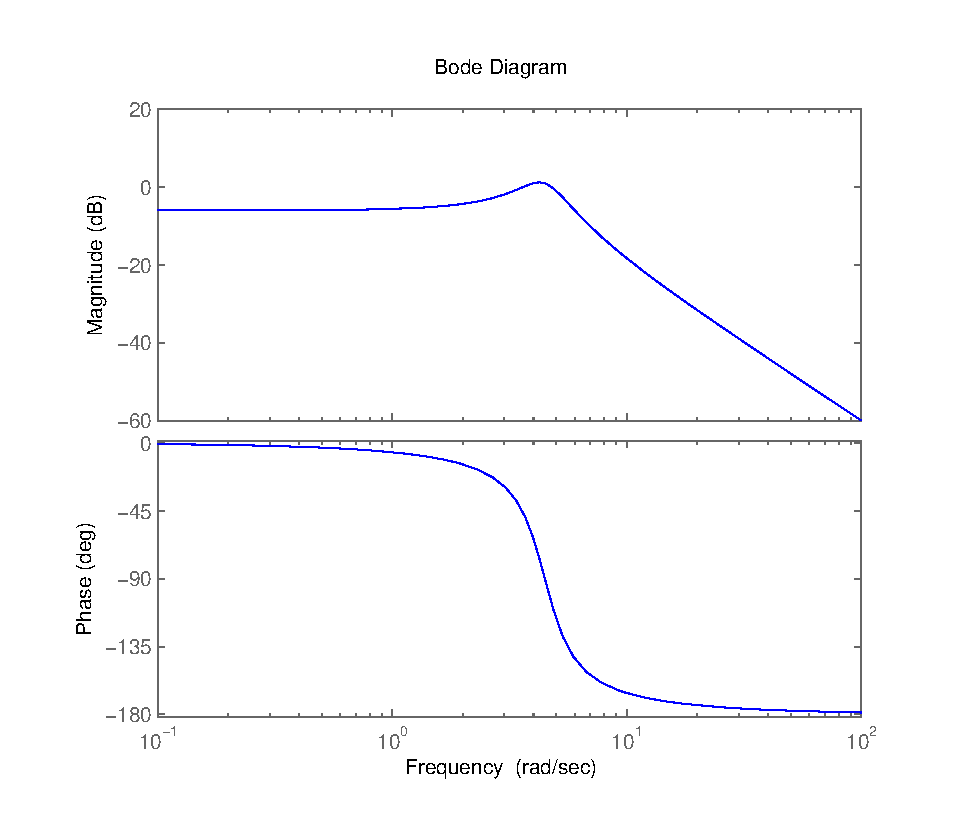
\includegraphics[width=0.98\columnwidth]{figures/bode_sem_ruido.eps}
	\caption{Diagrama de bode do sistema sem ruido.}
	\label{fig:bode_sem_ruido}
\end{figure}

\begin{figure}[htbp]
	\center
	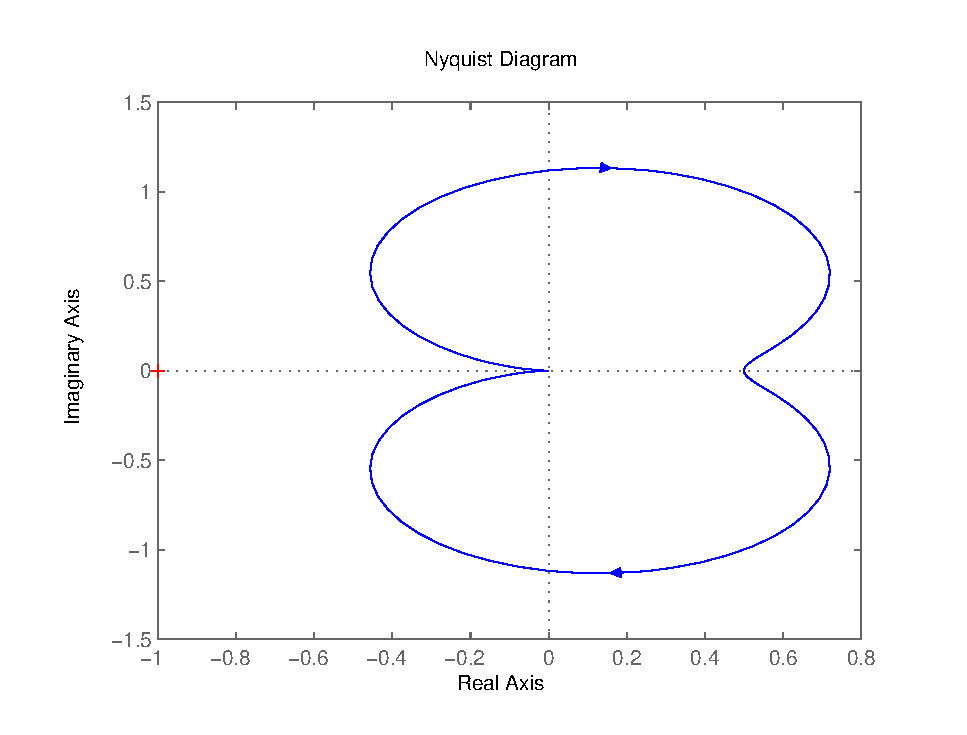
\includegraphics[width=0.98\columnwidth]{figures/nyquist_sem_ruido.eps}
	\caption{Diagrama de Nyquist do sistema sem ruido.}
	\label{fig:nyquist_sem_ruido}
\end{figure}

%===============================================================================
\subsection{M�todo B�sico}
\label{sec:bode_nyquest_basico}

Este m�todo simples consiste em aplicar uma onda senoidal na entrada do processo e observar qual
� a defasagem que a planta imp�em sobre a onde da entrada e a qual � o ganho de amplitude que 
� aplicado.

Como a planta em quest�o possui ru�do aditivo na sa�da, tem-se que as medidas efetuadas por este
m�todo s�o muito imprecisas, para calcular a amplitude do sinal de saida, basta analisar um ponto
que fique mediano ao ruido observado, mas para a fase, esta informa��o � mais complicada, pois como
a defasagem na planta em estudo � pequena, o ruido � muito grande, proporcionalmente, tornando as
medidas muito incertas.

Na Figura (\ref{fig:basic_method_1}) apresenta-se uma resposta padr�o para uma entrada senoidal.
Observa-se que a sa�da possui um ruido significante. Utilizando-se o mesmo procedimento, para diversas
frequ�ncias de ondas senoidais na entrada do processo, obt�m-se diversos pontos do diagrama de 
resposta em frequ�ncia do processo.

\begin{figure}[htbp]
	\center
	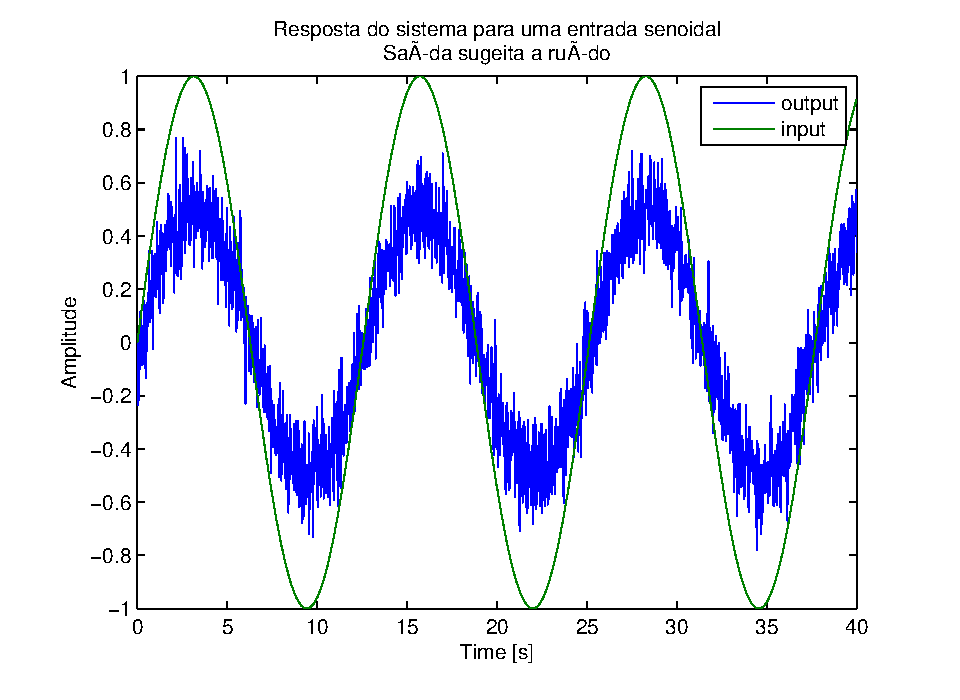
\includegraphics[width=0.98\columnwidth]{figures/basic_method_1.eps}
	\caption{Resposta do sistema para entrada senoidal}
	\label{fig:basic_method_1}
\end{figure}

Esta informa��es coletadas sobre o ganho e o deslocamento de fase aplicado sobre o sistema, chega-se as
informa��es que est�o contidas na Tabela (\ref{tab:basic_method})

\begin{table}[htbp]
  \begin{center}
	\caption{M�todo b�sico}
	\label{tab:basic_method}
	\begin{small}
	  \begin{tabular}{cll}
		\hline
		Frequ�ncia			& Ganho			& Fase [deg]	\\
		\hline
		0.01				& 0.5			& 0				\\
		0.1					& 0.45			& -11			\\
		0.5					& 0.5			& -46			\\
		1					& 0.55			& -14			\\
		5					& 0.85			& -86			\\
		10					& 0.14			& -200			\\
		50					& 0.13			& -186			\\
		100					& 0.0008		& -183			\\
		\hline
	  \end{tabular}
	\end{small}
  \end{center}
\end{table}

Os dados apresentados na Tabela (\ref{tab:basic_method}), podem ser utilizados para a confec��o 
do diagrama de bode do sistema apresentado na Figura (\ref{fig:bode_basic_method}). Observa-se que o formato
das curvas de fase e magnitude lembram as da Figura (\ref{fig:bode_sem_ruido}), mas a curva n�o
possui um fidelidade com a que caracteriza o sistema sem perturba��o.

\begin{figure}[htbp]
	\center
	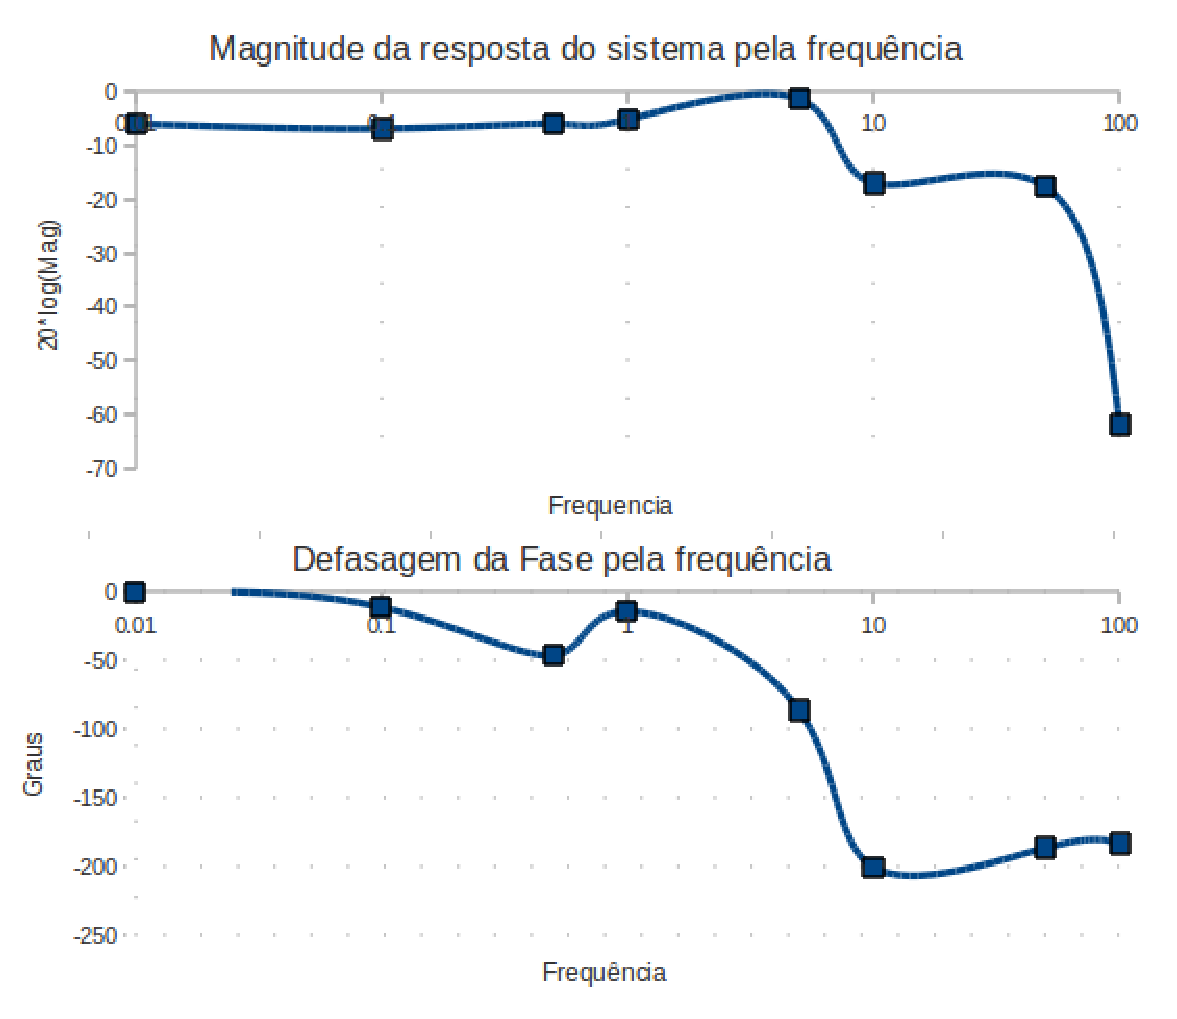
\includegraphics[width=0.98\columnwidth]{figures/basic_method.eps}
	\caption{Diagrama de Bode para o sistema sujeito a ruido, utilizando-se o m�todo b�sico para a 
	identifica��o da curva de resposta em frequ�ncia.}
	\label{fig:bode_basic_method}
\end{figure}
%===============================================================================
\subsection{M�todo melhorado}
\label{sec:bode_nyquest_melhorado}


\section{Resposta impulsiva}
\label{sec:resp_impulse}
%===============================================================================

A resposta impulsiva de um sistema consegue caracterizar por completo o comportamento de um
sistema para qualquer tipo de entrada. Pois convoluindo-se no tempo esta fun��o, com o 
sinal de entrada, tem-se o sinal de sa�da do sistema.

O objetivo nesta se��o � apresentar um m�todo para estimar-se esta resposta impulsiva do sistema.

Sabe-se que a equa��o apresentada em (\ref{eq:yt_h}) � verdadeira, que apresenta a convolu��o
do sinal discreto pela resposta impulsiva do sistema, acrescido de ruido.

\begin{equation}
y(t)=\sum_{k=0}^{\infty}h(k)u(t-k)+\nu (t)
\label{eq:yt_h}
\end{equation}

Em (\ref{eq:wiener_hopf}) tem-se a equa��o de Wiener-Hopf.

\begin{equation}
r_{yu}(\tau)=\sum_{k=0}^{\infty}h(k)r_u(\tau-k)
\label{eq:wiener_hopf}
\end{equation}

A fun��o covari�ncia em (\ref{eq:wiener_hopf}) pode ser obtida pelas equa��es (\ref{eq:ryu}) e
(\ref{eq:ru}).

\begin{equation}
\hat{r}_{yu}(\tau)=\frac{1}{N}\sum_{t=1}^{N-\tau}y(t+\tau)u(t)
\label{eq:ryu}
\end{equation}

\begin{equation}
\hat{r}_{u}(\tau)=\frac{1}{N}\sum_{t=1}^{N-\tau}u(t+\tau)u(t)
\label{eq:ru}
\end{equation}

Para $\tau = 0, 1, 2 ...$ e o sistema causal (y=0, para t <0).

Aplicando-se um sinal aleat�rio da entrada do sistema, a resposta impulsiva do mesmo 
pode ser obtida por (\ref{eq:h_noise}).

\begin{equation}
h(k)=\frac{r_{yu}(k)}{r_u(0)}
\label{eq:h_noise}
\end{equation}

Utilizando o c�digo do matlab apresentado no anexo 1, obteve-se a resposta impulsiva
apresentada na Figura (\ref{fig:h_impulse}). Na figura (\ref{fig:impulse}) apresenta-se 
a resposta impulsiva do sistema sem ruido, calculado pela fun��o Impulse do matlab.

\begin{figure}[htbp]
	\center
	\includegraphics[width=0.98\columnwidth]{figures/impulse_sem_ruido.eps}
	\caption{Resposta impulsiva do sistema sem a interfer�ncia do ruido, obtido utilizando a
	fun��o impulse do Matlab.}
	\label{fig:impulse}
\end{figure}

\begin{figure}[htbp]
	\center
	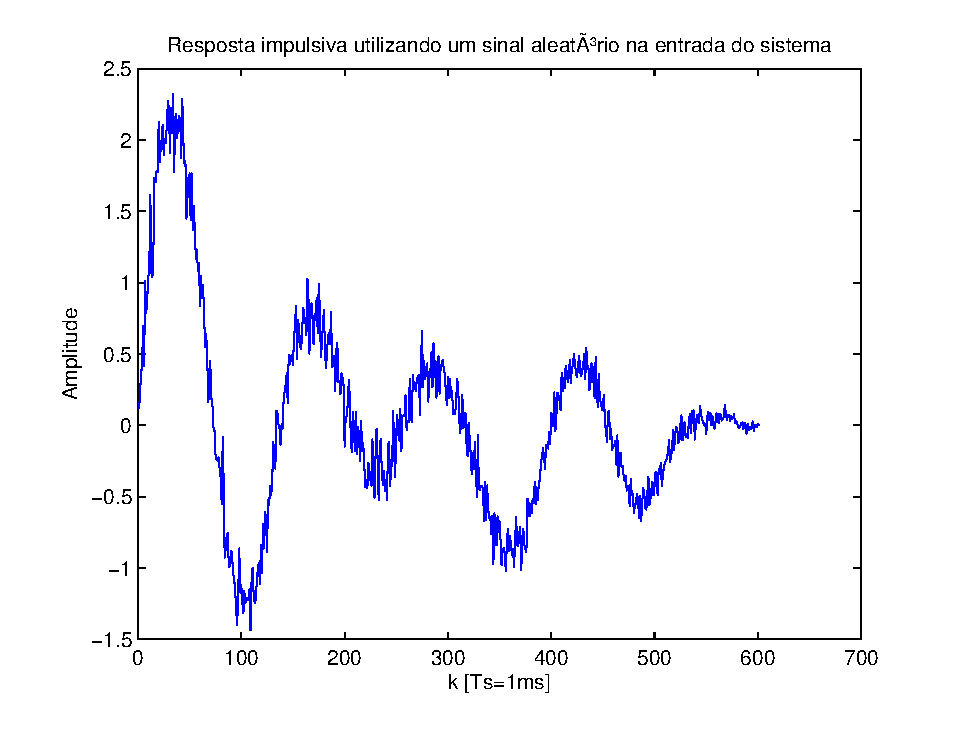
\includegraphics[width=0.98\columnwidth]{figures/impulse_com_ruido.eps}
	\caption{Resposta impulsiva do sistema com a interfer�ncia do ruido, obtido utilizando 
		um sinal aleat�rio na entrada do sistema.}
	\label{fig:h_impulse}
\end{figure}



\section{Conclus�es}
\label{sec:concl}

O projeto de controladores denominados Robustos � uma �rea bem abrangente e com
in�meras aplica��es na engenharia de controle. Sistemas sujeitos a incertezas s�o
praticamente todos os sistemas f�sicos, alguns com mais e outros com menos intensidade
e representatividade da incerteza apresentada. Estas incertezas como vimos pode ser
de v�rias origens (Se��o \ref{sec:caracterization}) e s�o classificadas em tipos. Neste
trabalho apresentamos a modelagem matem�tica de 4 tipos, considerados principais e
que cobrem boa parte das incertezas mais encontradas.

Incertezas do tipo polit�picas (Se��o \ref{sec:carac_politopica}) formam uma regi�o em forma de 
um politopo, e para se encontrar uma realimenta��o de estados para este sistema � 
necess�rio que o sistema seja est�vel em todos os v�rtices deste politopo. Nas se��es 
\ref{sec:normh2_politopico} e \ref{sec:hinf_sis_politopico} foi apresentado uma
realimenta��o de estados para incertezas deste tipo tendo como requisitos as normas 
$H_2$ e $H_{\infty}$ respectivamente. Foi observado pelas Figuras (\ref{fig:h2_polytopic})
e (\ref{fig:hinf_polytopic}) que o sistema que � submetido a norma $H_2$ possui um
sobrepasso maior para uma entrada do tipo degrau, e um tempo de acomoda��o maior
se comparado com o sistema sujeito a norma $H_{\infty}$.

Incertezas do tipo limitadas em norma (Se��o \ref{sec:carac_limit_norma}) onde n�o se tem 
informa��es detalhadas sobre os componentes do sistema. Para este tipo de incerteza se 
encontrou uma realimenta��o de estados sujeito as normas $H_2$ e $H_{\infty}$ e 
nas Figuras (\ref{fig:h2_norm_bounded}) e (\ref{fig:hinf_norm_bounded}) observa-se o
comportamento do sistema nos dois casos, com o sistema no centro das incertezas e tamb�m 
em algum dos v�rtices das incertezas.

Apresentou-se tamb�m a modelagem matem�tica para incertezas do tipo Diagonais 
(Se��o \ref{sec:carac_diagonais}) e elemento a elemento (Se��o \ref{sec:carac_elemento}).

Sa Se��o \ref{sec:robust} foi apresentado resumidamente a modelagem matem�tica utilizada
para resolver o problema de estabilidade dos sistemas sujeitos a cada uma das incertezas
retratadas neste trabalho.

Para a resolu��o dos problemas de incertezas para cumprimento das normas especificadas
foi utilizado o Solver de LMI \cite{lmi_matlab} do Matlab. A ferramenta � muito interessante e facilita 
muito o projeto e resolu��o da problem�tica que envolve sistemas mais complexos e com
mais incertezas em sua formula��o.

Controladores robustos s�o muitas vezes n�o s� desejados, mas tamb�m necess�rios em certos
tipos de aplica��es. Desta forma o estudo de modelagem, caracteriza��o e resolu��o destes
problemas se torna muito importante. O conhecimento matem�tico dos m�todos que as ferramentas
atuais utilizam para resolu��o dos problemas � tamb�m muito importante e �til para 
qualquer engenheiro que venha a se deparar com problemas incertos e com requisitos de
confiabilidade elevados.



%===============================================================================
\appendix
%===============================================================================
\chapter{1 - Script para Simula��o do MQ para o modelo ARX} 
\label{appendix_mmq}
\lstset{caption=M�todo dos m�nimos quadrados,label=DescriptiveLabel}
\lstinputlisting{matlab_files/simul.m}

%===============================================================================
\chapter{2 - Script para Simula��o do m�todo das vari�veis instrumentais} 
\label{appendix_iv}
\lstset{caption=M�todo das vari�veis instrumentais,label=DescriptiveLabel}
\lstinputlisting{matlab_files/simul_iv.m}

%===============================================================================
\chapter{3 - Script para Simula��o do m�todo dos minimos quadrados considerando o PID} 
\label{appendix_mmq_pid}
\lstset{caption=M�todo dos minimos quadrados considerando-se o controlador PID,label=DescriptiveLabel}
\lstinputlisting{matlab_files/simul_pid.m}

%===============================================================================



\bibliographystyle{IEEEtran}
\bibliography{biblio}

\end{document}
